\documentclass{TDP005mall}
\usepackage{graphicx}
\newcommand{\version}{Version 2.0}
\author{Agnes Hallberg, \url{agnha531@student.liu.se}\\
  Eric Jönsson, \url{erijo137@student.liu.se}}
\title{Designspecifikation}
\date{2018-12-19}
\rhead{Agnes Hallberg\\
  Eric Jönsson\\}
\begin{document}
\projectpage

\section*{Revisionshistorik}
\begin{table}[!h]
\begin{tabularx}{\linewidth}{|l|X|l|}
\hline
Ver. & Revisionsbeskrivning & Datum \\\hline
1.0 & Första utkast  & 18-11-27 \\\hline
2.0 & Redigerad version & 18-12-19 \\\hline
\end{tabularx}
\end{table}

\section{Detaljbeskrivning av Player}
Playerklassen ska representera karaktären spelaren kontrollerar. Spelaren har två olika attacker att välja mellan samt tre riktningar att röra sig i. Spelkaraktären kan inte lämna spelplanen. Klassen Player ärver från överklassen Entity. Vidare är Playerklassen vän till Swordklassen. Spelkaraktärens svärd är ett eget objekt och behöver ha tillgång till vad spelkaraktären gör i alla lägen. Följande klassmedlemmar finns i Playerklassen:
\begin{itemize}
\item int hp; ärvs från Entity. Denna datamedlem innehåller information om hur mycket skada spelkaraktären kan ta innan förlust.
\item Vector2f position; ärvs från Entity. Position sparar spelkaraktärens koordinater på banan.
\item Vector2f speed; ärvs från Entity. Dikterar hur snabbt spelkaraktären kan röra sig per tick.
\item Vector2f scale; ärvs från Entity. Bestämmer skalan på spelkaraktärens sprite.
\item Texture texture; ärvs från Entity. Anger vilken textur som ska sättas på spelkaraktärens sprite.
\item void player\_update(). Anropar underfunktioner för att kontrollera och uppdatera spelkaraktärens position, scale samt health. Denna funktion ansvarar även för att växla till Game Over-skärmen om spelkaraktärens health når 0.
\item void draw\_player(). Ritar ut spelkaraktärens sprite och textur på skärmen. Om spelkaraktären är immun mot skada ritas den till att blinka med en frekvens av 5 blink per sekund.
\item void process\_input(). Hanterar input från tangentbordet samt spelfönsterevents.
\item void collision(). Kontrollerar om spelkaraktären kolliderar med något fiendeobjekt och uppdaterar spelkaraktären enligt kontrollens resultat.
\item void hit(). Sänker spelkaraktärens health vid kollision med fiendeobjekt, såvida spelkaraktären inte är immun mot skada.
\item void jump(). Spelkaraktären rör sig i y-led till en viss y-koordinat och sedan tillbaka i motsatt riktning.
\end{itemize}
\section{Beskrivning av Enemy}
Enemyklassen ska reprensentera fienderna som spelaren behöver besegra. 
Enemyklassen har två underklasser; Peasant och Knight.
Enemy är en abstrakt klass. 
Spelkaraktären tar skada när den kolliderar med någon av fiendeobjekten. 
Fienderobjektens mål är att röra sig in i spelkaraktären. 
Enemyklassen ärver från Entityklassen.
\begin{itemize}
\item int hp; ärvs från Entity. Denna datamedlem innehåller information om hur mycket skada Enemyobjektet kan ta innan destruktion.
\item Vector2f position; ärvs från Entity. Position sparar Enemyobjektets koordinater på banan.
\item Vector2f speed; ärvs från Entity. Dikterar hur snabbt Enemyobjektet kan röra sig per tick.
\item Vector2f scale; ärvs från Entity. Bestämmer skalan på Enemyobjektets sprite.
\item Texture texture; ärvs från Entity. Anger vilken textur som ska sättas på Enemyobjektets sprite.
\item unsigned points. Anger hur mycket poäng Enemyobjektet ger spelaren vid destruktion.
\item int immunity. Används i hit() för att avgöra om Enemyobjektet tar skada eller inte.
\item void hit(). Denna funktion kallas när spelkaraktären träffar ett fiendeobjekt med en attack. Om attacken inte motsvarar värdet i immunity tar fienden skada.
\item void update(). Ansvarar för att Enemyobjekt rör sig mot spelkaraktären samt ritar Enemyobjektens sprite samt textur på spelskärmen.
\end{itemize}
\subsection{Peasant}
Peasant är den vanligaste förekommande fiendetypen. 
Peasant rör sig snabbare än spelkaraktären.
Vidare ärver Peasant all sin funktionalitet från Enemyklassen.
\subsection{Knight}
\begin{enumerate}
\item Knight ska upplevas svårare att besegra än Peasant. 
\item Knight rör sig långsammare än Peasant och spelkaraktären. 
\item Knights attack är långsam men kraftig.
\item Knight är immun mot svaga attacker. 
\item Knight kräver fler attacker för att besegras än andra fiendetyper.
\item Likt Playerklassen är Knightklassen en vän till Swordklassen. Detta för att Knightobjektets svärd fungerar precis som Playerobjektets svärd.
\end{enumerate}
\begin{itemize}
\item update(). Funktionen får Knightobjekt att följa spelkaraktären. Utöver detta får den Knightobjekten att starta sin attack när spelkaraktären är inom ett visst avstånd. Ansvarar även för att rita Knightobjektens sprite med textur samt det tillhörande Swordobjektet.
\end{itemize}

\newpage

Följande klassdiagram visar förhållandet mellan klasserna.
\begin{figure}[h!]
  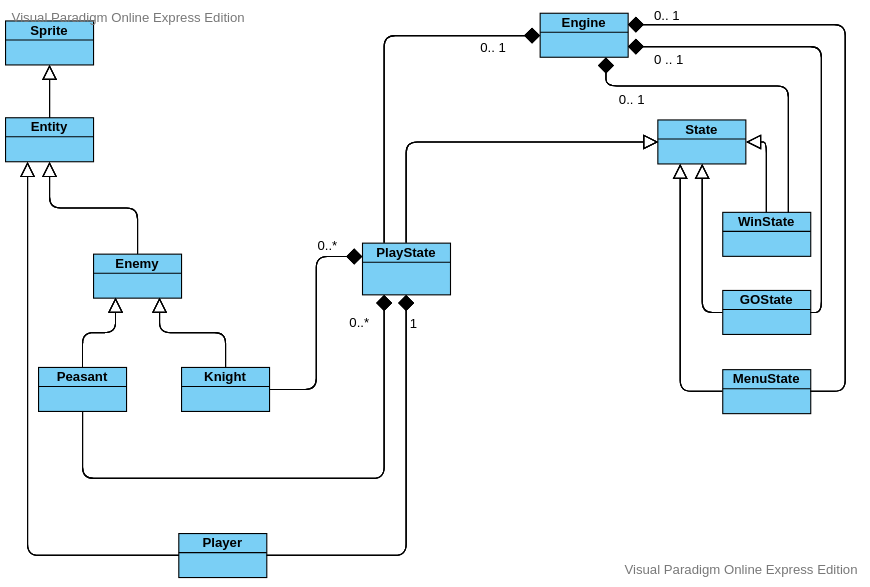
\includegraphics[width=\linewidth]{diagram.png}
  \caption{UML-diagram.}
\end{figure}

\newpage

\section{Designbeskrivning}
Designen av vårt spel bygger på att vi har en central spelmotor, Engine, som väljer mellan fyra olika spelstadier;
PlayState, MenuState, GameOverState samt WinState. Alla states ärver från basklassen State.
Vi gjorde detta designval för att enklare kunna expandera spelet med fler gamestates som till exempel cutscenes.


Vid växlingen skapas och förstörs de olika Statesobjekten. Vi har ingen pausfunktion i spelet och behöver därför inte bevara några Stateobjekt. Vi väljer att förstöra dem direkt när de slutas användas för att spara på hårdvaruresurser.

En uppenbar brist med detta designval är just att det blir omständigt att implementera en pausfunktion om den skulle önskas. Vi anser dock att det är emot spelets anda att ha en pausfunktion, då spelets ska upplevas svårt och oförlåtande. Dessutom är inte en spelomgång tänkt att vara tillräckligt lång för att rättfärdiga en pausfunktion. 

Då klasserna Player och Enemy har gemensamma attribut väljer vi att låta dem ärva från samma abstrakta klass, Entity. Detta leder till mindre upprepning av kod, vilket i sin tur leder till färre buggar och tydligare kod. Vi valde även att låta Entity ärva från SFML-bibliotekets inbyggda klass Sprite för att komma åt dess inbyggda funktioner, till exempel getPosition(). Detta sparade oss behovet att implementera egna funktioner för detta, vilket sparade mycket arbete. 

När spelet körs skapar det och visar ett MenuState. 
Via Menustate kan spelaren sedan skapa och växla till PlayState eller avsluta spelet.
När PlayState blir anropad får den information från Engine om vilka Enenmyobjekt som ska skickas in på spelplanen samt i vilken ordning. Engine i sin tur har läst in denna informationen från en extern fil.
PlayState sparar sedan Enemyobjekten i en egen vektor och behandlar all logik rörande fienderna, Engine och den externa filen är inte ansvariga i detta.

Vi valde att implementera detta för att göra skapandet samt modifierandet av fiendevågor simpelt. Designvalet gör det dessutom enklare för en oinsatt att modifiera fiendevågorna och skapa sina egna kombinationer av fiender.

En utbyggnad av denna designen hade varit att kunna välja mellan filer från MenuState. I skrivande stund kan spelets fiendekombination endast ändras genom att redigera den specifika filen, eller genom att ändra vilken fil som läses in av PlayState. Vid vidare utveckling av spelet hade vi gärna implementerat den funktionaliteten.

\section{Externa filer}
Spelet hanterar en extern txt-fil för att ladda in fiendevågor.   

\end{document}
